%%%%%%%%%%%%%%%%%%%%%%%%%%%%%%%%%%%%%%%%%
% Wenneker Article
% LaTeX Template
% Version 2.0 (28/2/17)
%
% This template was downloaded from:
% http://www.LaTeXTemplates.com
%
% Authors:
% Vel (vel@LaTeXTemplates.com)
% Frits Wenneker
%
% License:
% CC BY-NC-SA 3.0 (http://creativecommons.org/licenses/by-nc-sa/3.0/)
%
%%%%%%%%%%%%%%%%%%%%%%%%%%%%%%%%%%%%%%%%%

%----------------------------------------------------------------------------------------
%	PACKAGES AND OTHER DOCUMENT CONFIGURATIONS
%----------------------------------------------------------------------------------------

\documentclass[10pt, a4paper, twocolumn]{article} % 10pt font size (11 and 12 also possible), A4 paper (letterpaper for US letter) and two column layout (remove for one column)

%%%%%%%%%%%%%%%%%%%%%%%%%%%%%%%%%%%%%%%%%
% Wenneker Article
% Structure Specification File
% Version 1.0 (28/2/17)
%
% This file originates from:
% http://www.LaTeXTemplates.com
%
% Authors:
% Frits Wenneker
% Vel (vel@LaTeXTemplates.com)
%
% License:
% CC BY-NC-SA 3.0 (http://creativecommons.org/licenses/by-nc-sa/3.0/)
%
%%%%%%%%%%%%%%%%%%%%%%%%%%%%%%%%%%%%%%%%%

%----------------------------------------------------------------------------------------
%	PACKAGES AND OTHER DOCUMENT CONFIGURATIONS
%----------------------------------------------------------------------------------------

\usepackage[english]{babel} % English language hyphenation

\usepackage{microtype} % Better typography

\usepackage{amsmath,amsfonts,amsthm} % Math packages for equations

\usepackage[svgnames]{xcolor} % Enabling colors by their 'svgnames'

\usepackage[hang, small, labelfont=bf, up, textfont=it]{caption} % Custom captions under/above tables and figures

\usepackage{booktabs} % Horizontal rules in tables

\usepackage{lastpage} % Used to determine the number of pages in the document (for "Page X of Total")

\usepackage{graphicx} % Required for adding images

\usepackage{enumitem} % Required for customising lists
\setlist{noitemsep} % Remove spacing between bullet/numbered list elements

\usepackage{sectsty} % Enables custom section titles
\allsectionsfont{\usefont{OT1}{phv}{b}{n}} % Change the font of all section commands (Helvetica)

%\usepackage{url}
\usepackage{hyperref}
\usepackage{listings}
\usepackage[newfloat]{minted}
\usepackage{caption}

\definecolor{bg}{rgb}{0.9,0.9,0.9}

\newenvironment{code}{\captionsetup{type=listing}}{}
\SetupFloatingEnvironment{listing}{name=Snippet}

%----------------------------------------------------------------------------------------
%	MARGINS AND SPACING
%----------------------------------------------------------------------------------------

\usepackage{geometry} % Required for adjusting page dimensions

\geometry{
	top=1cm, % Top margin
	bottom=1.5cm, % Bottom margin
	left=2cm, % Left margin
	right=2cm, % Right margin
	includehead, % Include space for a header
	includefoot, % Include space for a footer
	%showframe, % Uncomment to show how the type block is set on the page
}

\setlength{\columnsep}{7mm} % Column separation width

%----------------------------------------------------------------------------------------
%	FONTS
%----------------------------------------------------------------------------------------

\usepackage[T1]{fontenc} % Output font encoding for international characters
\usepackage[utf8]{inputenc} % Required for inputting international characters

\usepackage{XCharter} % Use the XCharter font

%----------------------------------------------------------------------------------------
%	HEADERS AND FOOTERS
%----------------------------------------------------------------------------------------

\usepackage{fancyhdr} % Needed to define custom headers/footers
\pagestyle{fancy} % Enables the custom headers/footers

\renewcommand{\headrulewidth}{0.0pt} % No header rule
\renewcommand{\footrulewidth}{0.4pt} % Thin footer rule

\renewcommand{\sectionmark}[1]{\markboth{#1}{}} % Removes the section number from the header when \leftmark is used

%\nouppercase\leftmark % Add this to one of the lines below if you want a section title in the header/footer

% Headers
\lhead{} % Left header
\chead{\textit{\thetitle}} % Center header - currently printing the article title
\rhead{} % Right header

% Footers
\lfoot{} % Left footer
\cfoot{} % Center footer
\rfoot{\footnotesize Page \thepage\ of \pageref{LastPage}} % Right footer, "Page 1 of 2"

\fancypagestyle{firstpage}{ % Page style for the first page with the title
	\fancyhf{}
	\renewcommand{\footrulewidth}{0pt} % Suppress footer rule
}

%----------------------------------------------------------------------------------------
%	TITLE SECTION
%----------------------------------------------------------------------------------------

\newcommand{\authorstyle}[1]{{\large\usefont{OT1}{phv}{b}{n}\color{DarkRed}#1}} % Authors style (Helvetica)

\newcommand{\institution}[1]{{\footnotesize\usefont{OT1}{phv}{m}{sl}\color{Black}#1}} % Institutions style (Helvetica)

\usepackage{titling} % Allows custom title configuration

\newcommand{\HorRule}{\color{DarkGoldenrod}\rule{\linewidth}{1pt}} % Defines the gold horizontal rule around the title

\pretitle{
	\vspace{-30pt} % Move the entire title section up
	\HorRule\vspace{10pt} % Horizontal rule before the title
	\fontsize{32}{36}\usefont{OT1}{phv}{b}{n}\selectfont % Helvetica
	\color{DarkRed} % Text colour for the title and author(s)
}

\posttitle{\par\vskip 15pt} % Whitespace under the title

\preauthor{} % Anything that will appear before \author is printed

\postauthor{ % Anything that will appear after \author is printed
	\vspace{10pt} % Space before the rule
	\par\HorRule % Horizontal rule after the title
	\vspace{20pt} % Space after the title section
}

%----------------------------------------------------------------------------------------
%	ABSTRACT
%----------------------------------------------------------------------------------------

\usepackage{lettrine} % Package to accentuate the first letter of the text (lettrine)
\usepackage{fix-cm}	% Fixes the height of the lettrine

\newcommand{\initial}[1]{ % Defines the command and style for the lettrine
	\lettrine[lines=3,findent=4pt,nindent=0pt]{% Lettrine takes up 3 lines, the text to the right of it is indented 4pt and further indenting of lines 2+ is stopped
		\color{DarkGoldenrod}% Lettrine colour
		{#1}% The letter
	}{}%
}

\usepackage{xstring} % Required for string manipulation

\newcommand{\lettrineabstract}[1]{
	\StrLeft{#1}{1}[\firstletter] % Capture the first letter of the abstract for the lettrine
	\initial{\firstletter}\textbf{\StrGobbleLeft{#1}{1}} % Print the abstract with the first letter as a lettrine and the rest in bold
}

%----------------------------------------------------------------------------------------
%	BIBLIOGRAPHY
%----------------------------------------------------------------------------------------
\usepackage[super]{natbib}
%\usepackage[backend=bibtex,style=numbers,natbib=true]{biblatex}
%\usepackage[backend=bibtex,style=authoryear,natbib=true]{biblatex} % Use the bibtex backend with the authoryear citation style (which resembles APA)

\bibliographystyle{unsrtnat}

%\addbibresource{example.bib} % The filename of the bibliography

\usepackage[autostyle=true]{csquotes} % Required to generate language-dependent quotes in the bibliography
 % Specifies the document structure and loads requires packages

%----------------------------------------------------------------------------------------
%	ARTICLE INFORMATION
%----------------------------------------------------------------------------------------

\title{Towards Better Pixabay Tags} % The article title

\author{
	\authorstyle{Willie Maddox} % Authors
%	\authorstyle{Willie Maddox\textsuperscript{1,2,3}} % Authors
%	\newline\newline % Space before institutions
%	\textsuperscript{2}\institution{University of Texas at Austin, Texas, United States of America}\\ % Institution 2
%	\textsuperscript{3}\institution{\texttt{LaTeXTemplates.com}} % Institution 3
}

% Example of a one line author/institution relationship
%\author{\newauthor{John Marston} \newinstitution{Universidad Nacional Autónoma de México, Mexico City, Mexico}}

\date{\today} % Add a date here if you would like one to appear underneath the title block, use \today for the current date, leave empty for no date

%----------------------------------------------------------------------------------------

\begin{document}

\maketitle % Print the title

\thispagestyle{firstpage} % Apply the page style for the first page (no headers and footers)

%----------------------------------------------------------------------------------------
%	ABSTRACT
%----------------------------------------------------------------------------------------

\lettrineabstract{This document serves as the proposal for the final Capstone project for the Machine Learning Engineer Nanodegree offered through Udacity.}

%----------------------------------------------------------------------------------------
%	ARTICLE CONTENTS
%----------------------------------------------------------------------------------------

\section{Domain Background} % 1 - 2 para

% In this section, provide brief details on the background information of the domain from which the project is proposed. Historical information relevant to the project should be included. It should be clear how or why a problem in the domain can or should be solved. Related academic research should be appropriately cited in this section, including why that research is relevant.  Additionally, a discussion of your personal motivation for investigating a particular problem in the domain is encouraged but not required.

Pixabay is a website where photographers can publish and share copyright free images and videos.  Since all the contents are released under the CC0 license, they are safe to use without having to ask permission or give credit to the original artist. When a user submits a new image it must first be reviewed by the Pixabay admins.  They look at: 

\begin{itemize}
%	\item[Image Dimension] All images must have at least 1920 along the long dimension.
%	\item[Focus and Blurring] The image should be sharp and focused toward the center of the image.
%	\item[Light and Colors] Check that flash, if used, was used correctly and that image is not overexposed.
	\item Image Dimensions
	\item Focus and Blurring
	\item Lighting and Colors
	\item Copyright and Duplicates
	\item Image Manipulations
	\item Noise and JPEG Compression Artifacts
	\item Image Hygiene and Composition
	\item Tilted and Crooked Images
\end{itemize}

If the image satisfies the above categories then, most likely, it will be approved~\cite{Pixabay:Tagging}.  This is probably the primary reason Pixabay is so popular among photographers and artists alike; the overall quality of images in the database is professional grade.

\section{Problem Statement} % 1 para

Along with the image upload, the user must also provide at least 3 tags describing the content of the image.  The average number of tags per image is around 10.  Tags make the image easily searchable by other users.  Pixabay provides a tagging tutorial on their website but in general the tags are not required to meet the same level of quality standards that are placed on a newly uploaded image \citep{Pixabay:ImgStandards}. Nor can they really be enforced.  The metric for measuring the quality of an image is well defined.  All images must have at least 1920 along the long dimension.  The image should be sharp and in focus.  Avoid embedded timestamps.  These are all acceptable forms of objective measurement.  Tags, on the other hand, represent a persons description or interpretation of what is contained in an image and as such they are difficult to use as a source of measurement.  For example, Fig.\ref{screw-1924174_640} looks like a \textit{nuts and bolts} to me, but to someone else it might be \textit{hardware} or maybe even \textit{wood}.  Which tag is more \textit{correct} is unclear.  Hence, it is probably not a good idea to use tags as a measure of whether or not an image should or should not be approved. 

\begin{figure}
	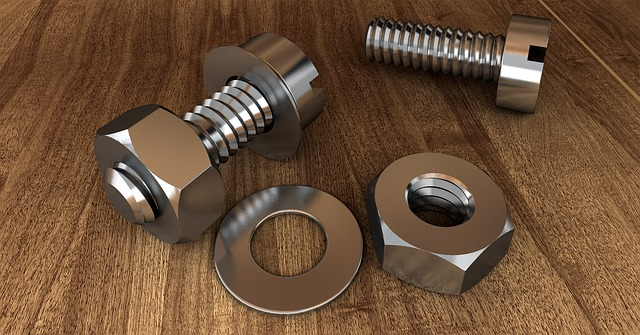
\includegraphics[width=\linewidth]{screw-1924174_640.jpg} % Figure image
	\caption{Nuts n Bolts n Boots n Pants} % Figure caption
	\label{screw-1924174_640} % Label for referencing with \ref{bear}
\end{figure}

When a user uploads an image to Pixabay, they are required to provide at least 3 labels (or tags) to describe the content of their image.  Assuming that the user is the original author (or photographer) of the image, then coming up with 3 relevant tags should be trivial.  However, on average, users will tend to choose around 10 tags to label their image, makeing it easier to find through searches.  

Incorrect search tags. papillon returns lots of butterflies (no papillon tag either)
Misspelled words, siberian husky not sibirian husky
People end up choosing tags that are not exactly relevant.
You don't have to spend a lot of time browsing pictures before you find one with a bogus label.
The problem is that many of the 


Can we improve the classification by adding more types of dogs, cats, etc.

The good thing is that users who upload pictures have first hand knowledge of familiar with the content in the image and can generally be trusted to tag the image correctly.  After all, an image with mislabeled tags is an image that no one will ever find. And since so much effort is required on the part of the author to get an image approved, it would seem highly unlikely that someone mislabel their own image on purpose.  

When a user is first presented with the tag screen, they are asked to type in tags corresponding to the content of their image.  After they type the first tag, a list of similar words (30 or so) appear for the user to select from. The list is auto-refreshed as new tags are added.  This is a nice convenience that Pixabay provides, but wouldn't it be even nicer to recommend to the user in the first place a list of tags based soley on the content of the image?  

In this section, clearly describe the problem that is to be solved. The problem described should be well defined and should have at least one relevant potential solution. 

Additionally, describe the problem thoroughly such that it is clear that the problem is:

\begin{description}
	\item[Quantifiable] The problem can be expressed in mathematical or logical terms.
	\item[Measurable] The problem can be measured by some metric and clearly observed.
	\item[Replicable] The problem can be reproduced and occurs more than once. Show examples of 2-3 images that have bogus tags.
\end{description}

\section{Datasets and Inputs} % 2 - 3 para

For this study we will use a custom Pixabay dataset as our primary dataset.  By custom we mean that we will only choose images with tags related to the 1000 classes in Imagenet.  We will also supplement our primary dataset with a secondary dataset consisting of both single-label and multi-label image datasets.  For single-label we will use Imagenet CLS-LOC\citep{ILSVRC15} dataset and for multi-label we will use the Imagenet DET\citep{ILSVRC15}, MSCOCO\citep{MSCOCO} and NUS-WIDE\citep{nus-wide-civr09} datasets.  These secondary datasets are very organized; they come with verified ground truth and can be easily downloaded and extracted for immediate use.  Data from Pixabay does not come prepackaged.  You must submit multiple search queries to build up your own database.  Fortunately they provide an API for registered users\citep{Pixabay:API}. The Pixabay API is well documented and it's usage is relatively straight forward.  At the minimum you need to pass it an API key for authentication and a query string of labels to search.  For example, to retrieve web format photos about "yellow flowers", the query string $q$ needs to be URL encoded\footnote{The key used in the url is invalid so don't expect it to work.  The url is meant to illustrate the basic structure of a request.}. \href{}{\nolinkurl{https://pixabay.com/api/?key=1234567-a1b2c3d4e5f6g7h8i9j0k1l2m&q=yellow+flowers&image_type=photo}}. The response for this request is a JSON encoded data structure containing metadata for a list of images.

\begin{code}
%\captionof{listing}{Pixabay API JSON response}
\caption{Pixabay API JSON response}
\label{snip:api-response}
\begin{minted}[bgcolor=bg]{json}
{
"total": 19177,
"totalHits": 500,
"hits": [
  {
    "id":2895728,
    "pageURL": ...,
    "type":"photo",
    "tags":"flower, pink, yellow",
    "previewURL": ...,
    "previewWidth":150,
    "previewHeight":112,
    "webformatURL": ...,
    "webformatWidth":640,
    "webformatHeight":480,
    "imageWidth":4608,
    "imageHeight":3456,
    "views":56,
    "downloads":25,
    "favorites":1,
    "likes":4,
    "comments":5,
    "user_id":5394567,
    "user":"GeorgeB2",
    "userImageURL": ...,
  },
  {
    "id": 195893,
    "tags": "blossom, bloom, flower",
    "webformatURL": ...,
    "..."
  },
  "..."
]
}
\end{minted}
\end{code}
\vspace{1mm}

A sample of the API response is shown in Snippet \ref{snip:api-response}.  There are three top level parameters: The \fcolorbox{white}{bg}{\textcolor{ForestGreen}{"total"}} number of images in the Pixabay database with tags matching the query, the maximum \fcolorbox{white}{bg}{\textcolor{ForestGreen}{"totalHits"}} that can be retrieved with the present query, and the actual \fcolorbox{white}{bg}{\textcolor{ForestGreen}{"hits"}} which are a list of python dictionaries, each containing metadata about a specific image in the database.  For our purposes, we only need a subset of this metadata:  A url to fetch the image, the set of labels that describe the image, and a mapping to help us keep track of which set of labels goes with each image.  Each "hit" contains a url for a low, medium, and high resolution version of an image. We choose the medium sized image \fcolorbox{white}{bg}{\textcolor{ForestGreen}{"webformatURL"}}. Since most pretrained models use images with dimensions between 200 and 300 pixels as input, this is an appropriate choice. As we can see in the code block, the \fcolorbox{white}{bg}{\textcolor{ForestGreen}{"tags"}} represent the labels for the image.  We will store the \fcolorbox{white}{bg}{\textcolor{ForestGreen}{"tags"}} in a dictionary using the \fcolorbox{white}{bg}{\textcolor{ForestGreen}{"id"}} as the key since they are unique across images. Each downloaded image will be saved using \fcolorbox{white}{bg}{\textcolor{ForestGreen}{"id"}} as the base of the file name.  So for the example above we will have 2895728.jpg and 195893.jpg.  This will make it easy to determine which image goes with which tags and vice versa.

The details (usage, directory layout, data formats, etc.) of the other datasets are available online and will not be discussed here.  However, it is worth mentioning how each of the datasets will be merged together. The syntax rules for labels depend on the dataset and are generally incompatable across datasets.  Some datasets capatilize proper nouns, some do not (Chihuahua vs chihuahua). Some use spaces to separate multi-word labels, others use underscores (golden retriever vs golden\_retriever). Some use alternate spellings (airplane vs aeroplane).  Before we can merge the above databases together into a complete database we will first need to decide on our own set of rules for labels.

\section{Solution Statement} % 1 para

%In this section, clearly describe a solution to the problem. The solution should be applicable to the project domain and appropriate for the dataset(s) or input(s) given. Additionally, describe the solution thoroughly such that it is clear that the solution is 

%\begin{description}
%	\item[Quantifiable] The solution can be expressed in mathematical or logical terms.
%	\item[Measurable] The solution can be measured by some metric and clearly observed.
%	\item[Replicable] The solution can be reproduced and occurs more than once.
%\end{description}

The solution is to train a model that is capable of generating a finite set of tags based solely on an input image.  We will measure the performance of our model by comparing the top $k$ predicted labels from our model against the known ground truth labels for each of our images.  The exact value of $k$ and the specific metric used are discussed in the following sections. We set aside a subset of our training data which will be used exclusively for testing. For each image in this testing set, the goal is to reproduce similar results for each one.

\section{Benchmark Model} % 1 - 2 para

% In this section, provide the details for a benchmark model or result that relates to the domain, problem statement, and intended solution. Ideally, the benchmark model or result contextualizes existing methods or known information in the domain and problem given, which could then be objectively compared to the solution. Describe how the benchmark model or result is measurable (can be measured by some metric and clearly observed) with thorough detail.

To benchmark the solution above, we will compare the testing set against three separate models.  The first one will simply be a pretrained Imagenet model\footnote{\url{https://keras.io/applications/}} (Just the base Imagenet model with 1000 classes. No fine tuning.) Since we will be using this same base model for transfer learning, we should expect similar performance classifing single-label images from the base Imagenet classes.  

For the second model, we will use Clarifai's image recognition API\footnote{\url{https://www.clarifai.com/}}.  Clarifai’s image recognition systems recognize various categories, objects, and tags in images, as well as find similar images. The company’s image recognition systems allow its users to find similar images in large uncategorized repositories using a combination of semantic and visual similarities.  We will use the evaluation metrics below to quantify how well the Clarifai model does on our training set.

The third benchmark model, Akiwi, is a semi-automatic image tagging system able to suggest keywords for uploaded images with minimal user input\footnote{\url{http://www.akiwi.eu/}}.  Akiwi does not offer a public API, instead you must drag and drop images in one at a time. We will most likely not run the entire testing set through this benchmark, but rather use it to study edge cases and outliers. It will be interesting to see how well our model compares to these state-of-the-art systems.

% J. Hartmann, N. Hezel, M. Krause and A. Sonnenberg under the supervision of Prof. Kai Uwe Barthel
% https://visual-computing.com/

\section{Evaluation Metrics} % 1 - 2 para

% In this section, propose at least one evaluation metric that can be used to quantify the performance of both the benchmark model and the solution model. The evaluation metric(s) you propose should be appropriate given the context of the data, the problem statement, and the intended solution. Describe how the evaluation metric(s) are derived and provide an example of their mathematical representations (if applicable). Complex evaluation metrics should be clearly defined and quantifiable (can be expressed in mathematical or logical terms).
There are two groups of evaluation metrics that apply to multi-label classification: \textit{example-based} metrics and \textit{label-based} metrics.
In regard to classification problems, there are a good many evaluation metrics to choose from. However, there are two in particular that are commonly used in multi-label classification problems.  The first is

The second is the Ja
\begin{equation}
\mathrm{IOU} = \frac{1}{N}\sum_{i=1}^{N}\frac{\vert y^i \wedge \hat{y} \vert}{\vert y^i \vee \hat{y} \vert}, \label{eq:IOU}
\end{equation}


\section{Project Design} % 1 page

% In this final section, summarize a theoretical workflow for approaching a solution given the problem. Provide thorough discussion for what strategies you may consider employing, what analysis of the data might be required before being used, or which algorithms will be considered for your implementation. The workflow and discussion that you provide should align with the qualities of the previous sections. Additionally, you are encouraged to include small visualizations, pseudocode, or diagrams to aid in describing the project design, but it is not required. The discussion should clearly outline your intended workflow of the capstone project.

Search for images with Imagenet Labels

There are restrictions that make getting the exact data you want a bit tricky.  For one, when you submit a query you get back a  

We will use WordNet to create consistent labels across the datasets.

Transfer learning on imagenet.  Add k classes where k is the number of classes in pixabay images that are not classified by Imagenet.

The training, validation, and testing datasets will be drawn from the complete dataset.

For this project, I will use a pretrained model of Imagenet

The plan is to use the Imagenet model as a fixed feature extractor

\begin{enumerate}
	\item How many images per category are there in Imagenet. (between 732 and 1300 per synset)
	\item How many nouns (or physical entities) are there in WordNet.
	\item How many hypernyms classes are there in Imagenet. 
	\item How many hyponyms per hypernym are there in Imagenet.
	\item What about holonyms and meronyms. Can they be of any use with this problem?
\end{enumerate}

Because the images are of such high quality on Pixabay they make great specimens for training on CNN's.

\begin{itemize}
	\item Tokenization
	\item Tagging - Nouns only
	\item Stemming
	\item Lemmatization
	\item Lexical semantics: synonym, antonym, hypernym, hyponym, meronym, holonym
	\item StopWord removal
\end{itemize}

$k-fold$ cross validation

too compensate for class imbalance, We will use stratification to construct the $k-fold$ cross validation subsets\citep{Kohavi_1995_1137, Sechidis2011}.


%----------------------------------------------------------------------------------------
%	BIBLIOGRAPHY
%----------------------------------------------------------------------------------------

\bibliography{example}
%\printbibliography[title={Bibliography}] % Print the bibliography, section title in curly brackets

%----------------------------------------------------------------------------------------

\end{document}
